\documentclass[14pt, a4paper]{extarticle}
\usepackage{GOST}
\usepackage{array}
\usepackage{verbatim}
\usepackage[detect-all]{siunitx}
\usepackage{amsmath}
\usepackage{amssymb}
\usepackage[utf8]{inputenc}
\usepackage{hyperref}
\usepackage{tempora}

\makeatletter
\renewcommand\@biblabel[1]{#1.}
\makeatother

\usepackage{listings}
\lstset{ 
	language=python,
	basicstyle=\small\sffamily, 
	numbers=left, 
	numberstyle=\tiny,
	stepnumber=1,
	numbersep=5pt,
	showspaces=false,            
	showstringspaces=false,      
	showtabs=false,             
	frame=single,            % рисовать рамку вокруг кода
	tabsize=4,      
	commentstyle=\color{green},
	keywordstyle=\color{blue}\textbf,
	numberstyle=\scriptsize\color{gray}, % the style that is used for the line-numbers
	rulecolor=\color{black},
	captionpos=t,
	breaklines=true,         % автоматически переносить строки 
	breakatwhitespace=false, % переносить строки по пробелу
	escapeinside={\#*}{*)} 
}

\begin{document}
	
\begin{table}[ht]
	\centering
	\begin{tabular}{|c|p{400pt}|} 
		\hline
		\begin{tabular}[c]{@{}c@{}} 
\includegraphics[scale=1]{source/b_logo.jpg} \\\end{tabular} &
		\footnotesize\begin{tabular}[c]{@{}c@{}}\textbf{Министерство~науки~и~высшего~образования~Российской~Федерации}\\\textbf{Федеральное~государственное~бюджетное~образовательное~учреждение}\\\textbf{~высшего~образования}\\\textbf{«Московский~государственный~технический~университет}\\\textbf{имени~Н.Э.~Баумана}\\\textbf{(национальный~исследовательский~университет)»}\\\textbf{(МГТУ~им.~Н.Э.~Баумана)}\\\end{tabular}  \\
		\hline
	\end{tabular}
\end{table}
\noindent\rule{\textwidth}{4pt}
\noindent\rule[14pt]{\textwidth}{1pt}
\hfill 
\noindent
\makebox{ФАКУЛЬТЕТ~}%
\makebox[\textwidth][l]{\underline{~«Информатика и системы управления»~~~~~~~~~~~~~~~~~~~~~~~~~~~~~~~~~}}%
\\
\noindent
\makebox{КАФЕДРА~}%
\makebox[\textwidth][l]{\underline{~«Программное обеспечение ЭВМ и информационные технологии»~}}%


\begin{center}
	\vspace{1.5cm}
	{\bf\huge Отчёт\par}
	{\bf\Large по лабораторной работе № 1\par}
	\vspace{0.7cm}
\end{center}

\noindent
\makebox{\large{\bf Название:}~~~}
\makebox[\textwidth][l]{\large\underline{~Программная  реализация приближенного~~~~~~~~~~~~~~~}}\\
\makebox[\textwidth][l]{\large\underline{~аналитического  метода  и численных алгоритмов  первого и~~~~~~~~~}}\\
\makebox[\textwidth][l]{\large\underline{~второго порядковточности при решении  задачи Коши для ОДУ.~}}


\noindent
\makebox{\large{\bf Дисциплина:}~~~}
\makebox[\textwidth][l]{\large\underline{~Моделирование~}}\\

\vspace{1.5cm}
\noindent
\begin{tabular}{l c c c c c}
	Студент      & ~ИУ7-65Б~               & \hspace{2.5cm} & \hspace{2cm}                 & &  Д.О. Склифасовский \\\cline{2-2}\cline{4-4} \cline{6-6} 
	\hspace{3cm} & {\footnotesize(Группа)} &                & {\footnotesize(Подпись, дата)} & & {\footnotesize(И.О. Фамилия)}
\end{tabular}

\noindent
\begin{tabular}{l c c c c}
	Преподователь & \hspace{5cm}   & \hspace{2cm}                 & & ~~~~~~~В.М. Градов~~~~~~~\\\cline{3-3} \cline{5-5} 
	\hspace{3cm}  &                & {\footnotesize(Подпись, дата)} & & {\footnotesize(И.О. Фамилия)}
\end{tabular}

\vspace{0.6cm}
\begin{center}	
	\vfill
	\large \textit {Москва, 2020}
\end{center}

\thispagestyle {empty}
\pagebreak

% ВВЕДЕНИЕ
\clearpage
\textbf{Цель работы:} получение навыков решения задачи Коши для ОДУ  методами Пикара и явными методами первого порядка точности (Эйлера) и второго порядка точности (Рунге-Кутта).
\section{Метод Пикара}
$y^{(1)}=\frac{x^3}{3}$

$y^{(2)}=\frac{x^3}{3} + \frac{x^7}{63}$

$y^{(3)}=\frac{x^3}{3}+ \frac{x^7}{63} + \frac{2x^{11}}{2079} + \frac{x^{15}}{59535}$

$y^{(4)}=\frac{x^3}{3}+ \frac{x^7}{63} + \frac{2x^{11}}{2079} + \frac{13x^{15}}{218295} + \frac{4x^{27}}{3341878155} + \frac{82x^{19}}{37328445} +  \frac{662x^{23}}{10438212015}$

$+\frac{x^{31}}{109876902975}$
\section{Метод Эйлера}
$y_{n+1}=y_n+h\cdot f(x_n,y_n)$, где$f(x,y)=x^2+y^2$
\section{Метод Рунге-Кутта}
\noindent$y_{n+1} = y_n + h ((1 - \alpha)k_1 + \alpha k_2)$\\
$k_1 = f(x_n, y_n)$\\
$k_2 = f(x_n + \frac{h}{2\alpha}, y_n + \frac{h}{2\alpha}k_1)$\\
$\alpha = \frac{1}{2}$ or $1$

\section*{Результаты}
\begin{figure}[h!]
	\centering{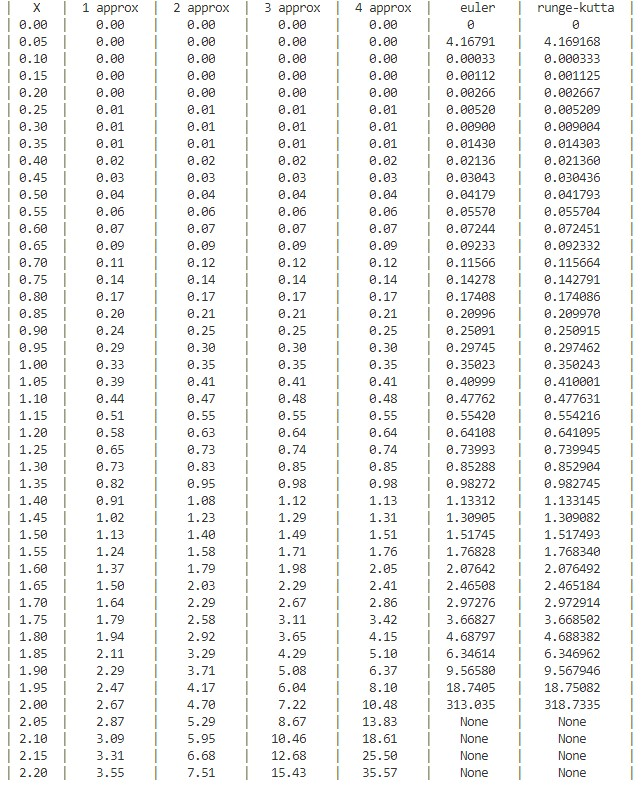
\includegraphics[scale=0.9]{source/result.jpg}}
\end{figure}
\newpage
\section*{Листинги}
\begin{lstlisting}[caption=Метод Пикара]
def pikar(approx, x):
	approximation = {
		1 : pow(x, 3) / 3.0,
		2 : pow(x, 3) / 3.0 + pow(x, 7) / 63.0,
		3 : pow(x, 3) / 3.0 + pow(x, 7) / 63.0 + 2 * pow(x, 11) / 2079.0
		+ pow(x, 15) / 59535.0,
		4 : pow(x, 3) / 3.0 + pow(x, 7) / 63.0 + 2 * pow(x, 11) / 2079.0
		+ 13 * pow(x, 15) / 218295.0 + 82 * pow(x, 19) / 37328445.0
		+ 662 * pow(x, 23) / 10438212015.0 + 4 * pow(x, 27) / 3341878155.0
		+ pow(x, 31) / 109876902975.0
	}
	return approximation.get(approx, "Invalid")
\end{lstlisting}
	
\begin{lstlisting}[caption=Метод Эйлера]
def euler(x, h):
	y = 0
	x0 = h
	while (x0 < x + h / 2):
		try:
			y += h * (pow(y, 2) + pow(x0, 2))
			x0 += h
		except:
			return 'None' 
	return y
\end{lstlisting}

\begin{lstlisting}[caption=Рунге-Кутта]
def runge_kutta(x, h, alpha):
	func = lambda x, u : pow(x, 2) + pow(u, 2)
	y = 0
	x0 = h
	while (x0 < x + h / 2):
		try:
			k1 = func(x0, y)
			k2 = func(x0 + h / (2 * alpha), y + h / (2 * alpha) * k1)
			y += h * ((1 - alpha) * k1 + alpha * k2)
			x0 += h
		except:
			return 'None'
	return y
\end{lstlisting}

\section*{Ответы на вопросы}
\begin{enumerate}
	\item[1)] Укажите интервалы значений аргумента, в которых можно считать решением заданного уравнения каждое из первых 4-х приближений Пикара. Точность результата ценивать до второй цифры после запятой. Обосновать свой ответ.\par
		\textbf{Ответ:} при оценке значений до 2-й цифры после запятой:
		\begin{itemize}
			\item Для первого - $[0, 0.65]$
			\item Для второго - $[0, 1.05]$
			\item Для третьего - $[0, 1.35]$
			\item Для четвертого - $[0, 1.35]$
		\end{itemize} 
		Из-за того, что нельзя точно гарантировать, что 4-ое приближение вычисляется верно (необходимо приближение более высокого порядка), интервалы 3-го и 4-го приближений одинаковые. \\
		Интервалы разные, так как, чем больше приближение, тем точнее результат.
	\item[2)] Пояснить, каким образом можно доказать правильность полученного результата при фиксированном значении аргумента в численных методах.\par
		\textbf{Ответ:} Численные методы работают итеративно, поэтому результаты зависят от величины шага. Необходимо выбирать такой шаг, при уменьшении которого результат будет меняться незначительно. В данной задании таким шагом является $10^{-5}$, так как значение не сильно отличается при шаге равном $10^{-6}$. Доказательство:
		
		\begin{table}[h]
			\begin{tabular}[scale=0.9]{|l|l|l|}\hline
				h & Эйлера  & Рунге-Кутта \\ \hline
				$10^{-3}$ & 142.627 & 431.1348 \\ \hline
				$10^{-4}$ & 277.362 & 327.977  \\ \hline
				$10^{-5}$ & 313.035 & 318.7335 \\ \hline
				$10^{-6}$ & 317.245 & 317.8234 \\ \hline     
			\end{tabular}
		\end{table}
	\item[3)] Какого значение функций при x=2, т.е. привести значение $u(2)$\par
		\textbf{Ответ:}
		\begin{table}[h]
			\begin{tabular}[scale=0.9]{|l|l|l|l|l|l|l|}\hline
				x & 1-e прибл. & 2-e прибл. & 3-e прибл. & 4-e прибл. & Эйлера  & Рунге-Кутта \\ \hline
				2.00 & 2.67   & 4.70    & 7.22  & 10.48  & 313.035  & 318.7335 \\ \hline     
			\end{tabular}
		\end{table}
\end{enumerate}








\end{document}









